\subsection{Comparadores}

Un comparador no es mas que un dispositivo capaz de establecer una relación de orden, esto es, un dispositivo capaz de determinar su una señal Va es por ejemplo mayor que Vb. El proceso de comparación puede ser reducido a una diferencia de señales (Va-Vb) y a la verificación del signo de dicha diferencia, si Va > Vb entonces el signo será positivo, si por el contrario Va < Vb entonces el signo será negativo. Esta forma de concebir una comparación sugiere la posibilidad de utilizar un amplificador operacional para implementar el dispositivo comparador \cite[pag. 2]{rivero-ao}.

La salida del dispositivo comparador es básicamente una variable booleana, por lo que también puede concebirse el comparador como una interfaz entre el mundo analógico y sistemas digitales.

\subsection{Comparador de lazo abierto}

El comparador de lazo abierto es el más simple de los comparadores, su funcionamiento se basa en la saturación del amplificador operacional. La saturación se produce cuando la diferencia de potencial entre las entradas inversora y no inversora es suficientemente grande como para que el amplificador no pueda seguir amplificando la señal. En este caso, la salida del amplificador se satura a uno de los dos valores de alimentación, dependiendo de la polaridad de la señal de entrada. La ilustración \ref{ilus:comparador-lazo-abierto} muestra este comportamiento.

\begin{ilustracion}[ht]
\centering
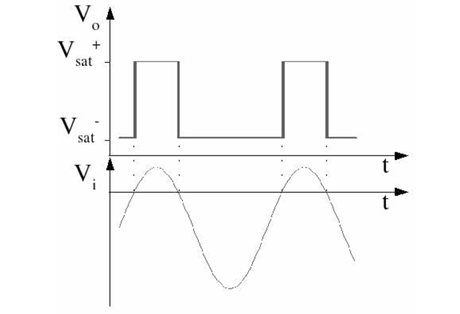
\includegraphics[width=0.5\textwidth]{marco-teorico/grafico-comparador-lazo-abierto.png}
\caption{Comparador de lazo abierto.}
\label{ilus:comparador-lazo-abierto}
\end{ilustracion}

Si el comparador fuese ideal, su salida seria exclusivamente dependiente de la polaridad de Vi respecto a tierra tal como se muestra en la ilustración \ref{ilus:comparador-lazo-abierto}.  Sin embargo debido a los desequilibrios de la etapa de entrada del comparador real (o del AO) se producirá una “tensión de ""offset"" de entrada”, tensión que puede variar entre un dispositivo y otro y que además es afectado con la temperatura y por la deriva temporal. Así entonces la salida del comparador no conmutara exactamente cuando la señal cruce por cero sino para alguna tensión en el rango (-Vos ,Vos) donde Vos no es mas que la máxima tensión de ""offset"" previsible.

Otro problema en la utilización de comparadores viene dado por el tiempo de respuesta, el cual puede determinarse como el tiempo transcurrido entre la aplicación de un flanco abrupto en la entrada diferencial y el momento en el cual la salida alcanza un alto porcentaje de su tensión en estado estacionario.

En la respuesta de salida que se muestra en la ilustración \ref{ilus:comparador-lazo-abierto-2} pueden distinguirse dos comportamientos claramente diferenciados, el primero es que en el cual aun habiéndose producido un cambio en la entrada, la salida no cambia en lo absoluto durante un tiempo td (delay) o de retardo, pasado este tiempo la señal de salida cambia paulatinamente alcanzando una rata de ascenso que viene dada por el Slewrate.

\begin{ilustracion}[ht]
  \centering
  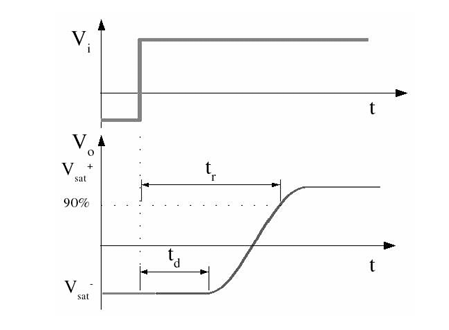
\includegraphics[width=0.5\textwidth]{marco-teorico/respuesta-comparador-a-franco.png}
  \caption{Respuesta de un comparador de lazo abierto a un flanco abrupto.}
  \label{ilus:comparador-lazo-abierto-2}
\end{ilustracion}

Otro problema inherente a los comparadores a lazo abierto es producido por el ruido que inevitablemente acompaña a la señal de entrada. Suponiendo una señal de entrada contaminada por ruido(aditivo) tal como la que se muestra en la ilustración \ref{ilus:comparador-lazo-abierto-3}, en este caso la salida del comparador no será una señal cuadrada sino que estará contaminada por el ruido.

\begin{ilustracion}[ht]
  \centering
  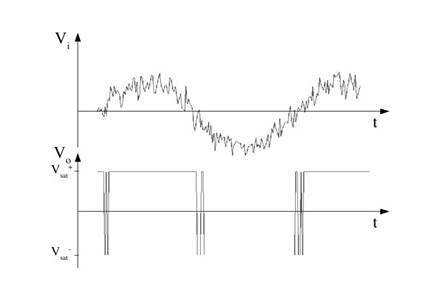
\includegraphics[width=0.5\textwidth]{marco-teorico/respuesta-comparador-a-ruido.png}
  \caption{Respuesta de un comparador de lazo abierto a una señal de entrada contaminada por ruido.}
  \label{ilus:comparador-lazo-abierto-3}
\end{ilustracion}

\subsection{Comparador de lazo cerrado}

Los comparadores también pueden ser realimentados, solo que en su caso resulta mucho más beneficiosa la realimentación positiva en zona lineal, que la negativa como es usual en los A.O. Al practicar realimentación positiva en un comparador se obtiene fundamentalmente un nuevo comportamiento conocido como histéresis, en el cual los niveles de conmutación cambian con el estado (el nivel de tensión) en el que se encuentra el comparador. Ahora el circuito tiene dos niveles de umbral diferentes para la señal de entrada, uno para la transición de bajo a alto y otro para la transición de alto a bajo. Esta característica hace que el comparador de lazo cerrado sea muy útil para eliminar el ruido en las señales y para convertir una señal analógica en una señal digital. \cite[pag. ]{rivero-ao}

\subsection{Osciladores de relajación}

Estos osciladores utilizan dispositivos biestables, como interruptores, disparadores Schmitt, compuertas lógicas y flip-flops, para cargar y descargar repetidamente un capacitor. Las formas de onda típicas que se pueden obtener con este método son las ondas triangular, de diente de sierra, exponencial, cuadrada y de pulso. A medida que avancemos, a menudo necesitaremos calcular el tiempo $\Delta t$ que tarda en cargarse (o descargarse) un capacitor en una cantidad dada $\Delta v$. Las dos formas más comunes de carga/descarga son la lineal y la exponencial. \cite[pag. 484]{sergio-franco}

Cuando se alimenta con una corriente constante I, un capacitor C se carga o descarga a una tasa constante, produciendo un transitorio lineal o rampa del tipo mostrado en la Ilustración \ref{ilus:carga-descarga-lineal}. Los ingenieros suelen describir esta rampa mediante la relación fácil de recordar:

\begin{equation}
  C \Delta v = I \Delta t
\end{equation}

De donde se puede despejar el tiempo de carga o descarga:

\begin{equation}
  \Delta t = \frac{C }{I} \Delta v
  \label{eq:tiempo_carga-lineal}
\end{equation}

\begin{ilustracion}[ht]
  \centering
  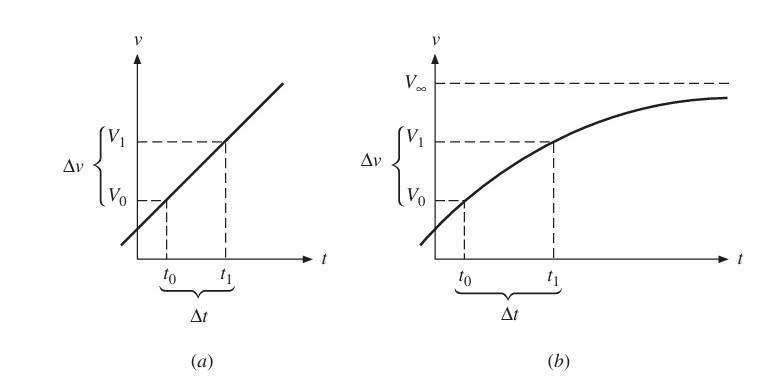
\includegraphics[width=0.5\textwidth]{marco-teorico/carga-condensador.png}
  \caption{Carga y descarga lineal y exponencial de un capacitor.}
  \label{ilus:carga-descarga-lineal}
\end{ilustracion}

Un \emph{transitorio exponencial} ocurre cuando $C$ se carga o descarga a través de una resistencia en serie $R$. Con referencia a la Fig. 10.1b, el voltaje instantáneo en el capacitor está dado por:

\[
v(t) = V_\infty + (V_0 - V_\infty) \exp[-(t - t_0)/\tau]
\]

donde:
\begin{itemize}
\item $V_0$ es el voltaje inicial,
\item $V_\infty$ es el voltaje en estado estacionario que se alcanzaría en el límite $t \to \infty$,
\item $\tau = RC$ es la constante de tiempo que gobierna el transitorio.
\end{itemize}

Esta ecuación es válida independientemente de los valores y polaridades de $V_0$ y $V_\infty$. El transitorio alcanza un valor intermedio especificado $V_1$ en un instante $t_1$ tal que:

\[
V_1 = V_\infty + (V_0 - V_\infty) \exp[-(t_1 - t_0)/\tau]
\]

Tomando el logaritmo natural a ambos lados y despejando $\Delta t = t_1 - t_0$, podemos estimar el tiempo que tarda en cargarse o descargarse $C$ desde $V_0$ hasta $V_1$ como:

\begin{equation}
\Delta t = \tau \ln \frac{V_{\infty} - V_0}{V_{\infty} - V_1}
\label{eq:tiempo_carga-exponencial}
\end{equation}

\subsection{Multivibradores}

Los multivibradores son circuitos regenerativos diseñados especialmente para aplicaciones de temporización y generación de formas de onda. Los multivibradores 
pueden generar señales de salida que cambian entre dos estados, lo que los hace útiles para una variedad de aplicaciones, incluyendo osciladores, temporizadores, y flip-flops.

\subsubsection{Multivibrador astable}

El multivibrador astable conmuta espontáneamente entre un estado y otro, sin necesidad de comandos externos. También conocido como \emph{multivibrador auto-oscilante}, su frecuencia está determinada por una red adecuada, que generalmente incluye:

\begin{itemize}
    \item Un capacitor (para oscilaciones RC)
    \item Un cristal de cuarzo (para mayor precisión)
\end{itemize}

Características principales:
\begin{itemize}
    \item No posee estados estables (de ahí el término "astable")
    \item Genera ondas cuadradas continuamente
    \item La frecuencia depende de los valores de los componentes pasivos
\end{itemize}

\begin{ilustracion}[ht]
  \centering
  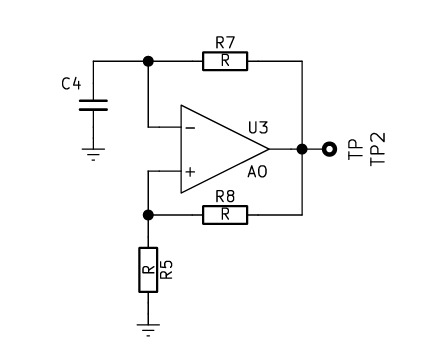
\includegraphics[width=0.8\textwidth]{marco-teorico/multivibrador-astable.png}
  \caption
  {Multivibrador astable.}
  \label{ilus:multivibrador-astable}
\end{ilustracion}

En el circuito de la ilustración \ref{ilus:multivibrador-astable}-a, el comparador de amplificador operacional y las resistencias de retroalimentación positiva \( R_1 \) y \( R_2 \) forman un \emph{disparador Schmitt inversor}. Asumiendo una saturación simétrica de salida en \(\pm V_{\text{sat}}, \text{V}\), los umbrales del disparador Schmitt también son simétricos:

\[
\pm V_T = \pm V_{\text{sat}} \frac{R_1}{R_1 + R_2} 
\]

La señal a la entrada inversora es provista por el propio amplificador operacional a través de la red RC.

Al encender la alimentación (\( t = 0 \)), \( v_O \) cambiará a \(+V_{\text{sat}}\) o \(-V_{\text{sat}}\), ya que estos son los únicos estados estables permitidos por el disparador Schmitt. Suponiendo que cambia a \(+V_{\text{sat}}\), se tendrá \( v_P = +V_T \). Esto hará que \( R \) cargue \( C \) hacia \( V_{\text{sat}} \), produciendo un aumento exponencial en \( v_N \) con constante de tiempo \( \tau = RC \). Cuando \( v_N \) alcanza \( v_P = V_T \), \( v_O \) cambia abruptamente a \(-V_{\text{sat}}\), invirtiendo la corriente del capacitor y haciendo que \( v_P \) cambie a \(-V_T\). Luego, \( v_N \) decae exponencialmente hacia \(-V_{\text{sat}}\) hasta alcanzar \( v_P = -V_T \), momento en el que \( v_O \) vuelve a \(+V_{\text{sat}}\), repitiéndose el ciclo. Claramente, el circuito puede iniciar y mantener una oscilación, con \( v_O \) alternando entre \(+V_{\text{sat}}\) y \(-V_{\text{sat}}\), y \( v_N \) variando exponencialmente entre \(+V_T\) y \(-V_T\). Después del ciclo inicial, las formas de onda se vuelven periódicas. \cite[pag. 492]{sergio-franco}

La frecuencia de oscilación \( f_0 \) se determina a partir del periodo \( T \) como \( f_0 = 1/T \). Debido a la simetría de los niveles de saturación, \( v_O \) tiene un ciclo de trabajo del 50\%, por lo que solo es necesario calcular \( T/2 \). Aplicando la Ec. (10.3) con \( \Delta t = T/2 \) y \( \tau = RC \):

\[
\frac{T}{2} = \tau \ln \left( \frac{V_{\infty} - V_0}{V_{\infty} - V_1} \right)
\]

donde:
\begin{itemize}
    \item \( V_{\infty} = V_{\text{sat}} \)
    \item \( V_0 = -V_T \)
    \item \( V_1 = +V_T \)
    \item \( \tau = RC \)
\end{itemize}

Sustituyendo los valores simétricos:

\[
\frac{T}{2} = RC \ln \left( \frac{V_{\text{sat}} - (-V_T)}{V_{\text{sat}} - V_T} \right) = RC \ln \left( \frac{V_{\text{sat}} + V_T}{V_{\text{sat}} - V_T} \right)
\]

Finalmente, la frecuencia de oscilación es:

\[
f_0 = \frac{1}{2RC \ln \left( \frac{V_{\text{sat}} + V_T}{V_{\text{sat}} - V_T} \right)}
\]


\subsubsection{Multivibrador monoestable}

El multivibrador monoestable genera pulsos de ancho $T$ al ser disparado, implementable con: (a) Contadores digitales o (b) Redes RC ($T \approx 1.1RC$ para CI 555). Aplicaciones incluyen generación de retardos, señales de habilitación y eliminación de rebotes en interruptores. \cite[pag. 498]{sergio-franco}

El multivibrador monoestable tiene un estado estable en el que puede permanecer indefinidamente. También tiene un estado cuasiestable al que puede ser activado (o disparado) y en el que permanece durante un intervalo predeterminado, igual al ancho deseado del pulso de salida. Cuando este intervalo termina, el multivibrador monoestable regresa a su estado estable y permanece allí, esperando otra señal de activación (o disparo). \cite[pag. 1368]{sedra-smith}

\begin{ilustracion}[ht]
  \centering
  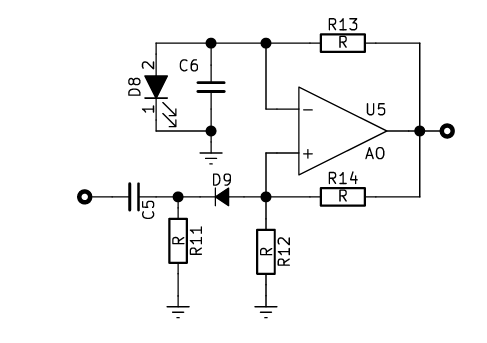
\includegraphics[width=0.8\textwidth]{marco-teorico/multivibrador-monostable.png}
  \caption
  {Multivibrador monoestable.}
  \label{ilus:multivibrador-monoestable}
\end{ilustracion}

La ilustración \ref{ilus:multivibrador-monoestable}-a muestra un circuito monoestable basado en un amplificador operacional (op-amp). Se observa que este circuito es una versión modificada del circuito astable de la ilustración \ref{ilus:multivibrador-astable}. En concreto, se ha añadido un diodo de sujeción \( D_1 \) en paralelo con el capacitor \( C_1 \), y un circuito de disparo compuesto por el capacitor \( C_2 \), la resistencia \( R_4 \) y el diodo \( D_2 \) se conecta a la entrada no inversora del op-amp. \cite[pag. 1368]{sedra-smith}

El circuito opera de la siguiente manera:

\begin{itemize}
    \item \textbf{Estado estable}: En ausencia de una señal de disparo, la salida del op-amp está en \( L_+ \), y el diodo \( D_1 \) conduce a través de \( R_3 \), fijando el voltaje \( v_B \) a una caída de diodo por encima de tierra. Se elige \( R_4 \) mucho mayor que \( R_1 \), de modo que \( D_2 \) conduzca una corriente muy pequeña y el voltaje \( v_C \) quede determinado principalmente por el divisor de tensión \( R_1 \), \( R_2 \). Así, \( v_C = \beta L_+ \), donde \( \beta = \frac{R_1}{R_1 + R_2} \). Este estado se mantiene porque \( \beta L_+ \) es mayor que \( V_{D1} \).

    \item \textbf{Disparo}: Al aplicar un flanco negativo en la entrada de disparo (ver formas de onda en ilustración \ref{ilus:multivibrador-monoestable}-b), este acopla un voltaje negativo al cátodo de \( D_2 \) a través de \( C_2 \), haciendo que \( D_2 \) conduzca fuertemente y lleve el nodo \( C \) a un nivel bajo. Si la señal de disparo es suficientemente grande para que \( v_C \) caiga por debajo de \( v_B \), el op-amp detectará una tensión negativa neta en su entrada y su salida cambiará a \( L_- \). Esto, a su vez, hará que \( v_C \) pase a \( \beta L_- \), manteniendo el op-amp en este nuevo estado. En este punto, \( D_2 \) se corta, aislando el circuito de cambios posteriores en la entrada de disparo.

    \item \textbf{Estado cuasiestable}: El voltaje negativo en \( A \) corta \( D_1 \), y \( C_1 \) comienza a descargarse exponencialmente hacia \( L_- \) con una constante de tiempo \( C_1 R_3 \). El multivibrador permanece en este estado hasta que \( v_B \) cae por debajo de \( \beta L_- \). En ese instante, la salida del op-amp vuelve a \( L_+ \), y \( v_C \) retorna a \( \beta L_+ \). El capacitor \( C_1 \) se recarga entonces hacia \( L_+ \) hasta que \( D_1 \) conduce nuevamente, restaurando el estado estable.
\end{itemize}